%
% latex-sample.tex
%
% This LaTeX source file provides a template for a typical research paper.
%

%
% Use the standard article template.
%
\documentclass{article}

% The geometry package allows for easy page formatting.
\usepackage{geometry}
\geometry{letterpaper}

% Load up special logo commands.
\usepackage{doc}
%\usepackage[utf8]{inputenc}
\usepackage[english]{babel}

\usepackage{amsthm}
 
\newtheorem*{remark}{Remark}
\newtheorem{example}{Example}

\usepackage{multirow}
\usepackage[table]{xcolor}

% itemize in table
\usepackage{booktabs}
\newcommand{\tabitem}{~~\llap{\textbullet}~~}
\usepackage{tabularx}
\usepackage{paralist}
\usepackage{pifont}
\usepackage{array}
\usepackage{longtable}

% Package for formatting URLs.
\usepackage{url}
\usepackage{float}

% Packages and definitions for graphics files.
\usepackage{graphicx}
\usepackage{epstopdf}
\usepackage{color}
\DeclareGraphicsRule{.tif}{png}{.png}{`convert #1 `dirname #1`/`basename #1 .tif`.png}

% Source code
%% minted package
\usepackage{minted}
\newminted{sql}{mathescape, linenos, numbersep=5pt, gobble=0, frame=lines, framesep=2mm}

%% listing package
\usepackage{listings}
\lstset{language=SQL}
\usepackage{caption}
\DeclareCaptionFont{white}{\color{white}}
\DeclareCaptionFormat{listing}{\colorbox{gray}{\parbox{\textwidth}{#1#2#3}}}
\captionsetup[lstlisting]{format=listing,labelfont=white,textfont=white}

%
% Set the title, author, and date.
%
\title{DB2 Exam 610 Summary}
\author{Zeyuan Hu}
\date{\today}

% set indentation of paragraph
\setlength{\parindent}{0em}

%
% The document proper.
%
\begin{document}

% Add the title section.
\maketitle

% Add an abstract.
% \abstract{}

% Add various lists on new pages.
\pagebreak
\tableofcontents

% \pagebreak
% \listoffigures

% \pagebreak
% \listoftables

% Start the paper on a new page.
\pagebreak

%
% Body text.
%
\section{Planning}
\label{planning}

\subsection{Objectives}
\label{objectives}

\begin{itemize}
\item Knowledge of DB2 products (z/OS vs LUW vs pureScale - at a high-level; different products 
and what they do)
\item Knowledge of database workloads (appropriate DB2 product to use - OLTP vs warehousing)
\item Knowledge of non-relational data concepts (XML data, LOB data)
\end{itemize}

\subsection{Database workloads}
\label{database workloads}

Two main types of database application workloads:
\begin{itemize}
\item online transactional processing (OLTP)
\item data warehousing
\begin{itemize}
\item reporting
\item online analytical processing (OLAP)
\item data mining applications
\item decision support
\end{itemize}
\end{itemize}

\subsection{OLTP vs. Data Warehousing}
\label{oltp vs. data warehousing}

An OLTP system is typical of a web order system, where you perform transactions over the web
(such as ordering a product). Online transaction processing (OLTP) systems features:

\begin{itemize}
\item Support day-to-day, mission-critical business activities (ie. web-based order entry, stock trading)
[\textit{current data}]
\item Support hundreds to thousands of users issuing millions of transactions per day
against databases that vary in size [\textit{Frequent updates, Granular transactions}]
\item Response time requirements tend to be subsecond [\textit{Sub-second response time}]
\item Queries:
\begin{itemize}
\item tend to be a mix of real-time insert, update, and delete
operations against current-as opposed to historical-data
\item single-row lookups with logic that likely updates a small number of records
\end{itemize}
\end{itemize}


Data warehousing system typically consist of:
\begin{itemize}
\item Store and manage large volumes of data that is often historical in nature and is used primarily for
analysis [\textit{Voluminous historical data}]
\item Optimized for queries
\item Heterogeneous data sources
\item Queries: (ie. [\textit{Summarized queries that perform aggregations and joins}] )
\begin{itemize}
\item bulk load operations
\item short-running queries
\item long-running complex queries
\item random queries
\item occasional updates to data
\item execution of online utilities
\end{itemize}

\end{itemize}

\begin{example}
A database will be used primarily to identify sales patterns for products sold within the 
last three years and to summarize sales by region, on a quarterly basis. In case, a Data warehouse 
system is needed.
\end{example}

\begin{remark}
Different by {\color{red} queries that are typically used to access the data} (aka workloads).
\end{remark}


\begin{figure}[h]
\centering
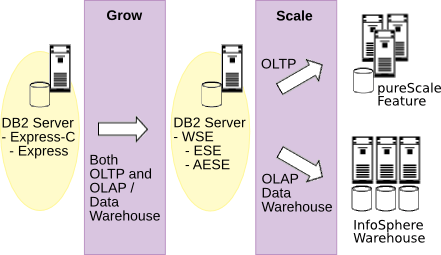
\includegraphics[scale=0.4]{workloads.png}
 
\caption{DB2 products, OLTP, Data Warehouse}
\label{workloads}
\end{figure}

\subsection{DB2 pureScale - IBM solution for OLTP}
\label{DB2 pureScale}

\medskip

System highlights:
\begin{itemize}
\item Best suited for OLTP workloads
\item Enables a \texttt{DB2 for LUW} database to continously process incoming requests, even if
multiple system components fail simultaneously, which makes it ideal for OLTP workloads where high
availability is crucial
\item Provides a database cluster solution for nonmainframe platforms
\item Can \textbf{ONLY} work with the General Parallel File System (GFPS) file system
\end{itemize}

\medskip

Usage:
\begin{itemize}
\item Can be used with \texttt{DB2 Workgroup Server Edition (WSE)}, \texttt{DB2 Enterprise Server Edition
(ESE)}, \texttt{DB2 Advanced Enterprise Server Edition(AESE)}
\item Can \textbf{ONLY} be installed on IBM p Series or x Series servers that are running either
the AIX (p Series) or the Linux (x Series) operating system
\item \textbf{CANNOT} be installed on IBM mainframes running z/OS, IBM p Series server running Linux,
or IBM x Series servers running Windows
\end{itemize}


\subsection{InfoSphere Warehouse - IBM solution for Data warehousing}

\medskip
System highlights:
\begin{itemize}
\item is a complete data warehousing solution that contains components that facilitate
data warehouse construction and administration, as well as tools that enable embedded data
mining and multidimensional online analytical processing (OLAP)
\end{itemize}

\subsection{Notable DB2 features \& products}

\textbf{IBM Data Studio}
\begin{itemize}
\item is an Eclipse-based, integrated development environment (IDE) that can be used to perform
instance and database administration, routine (SQL procedure, SQL functions, etc.) and application
development, and performance-tuning tasks.
\item replaces the \texttt{DB2 Control Center} as the standard GUI tool for DB2 database administration
and application development.
\item allows users to connect to a DB2 database using a wizard; however, users are required to provide
login credentials before a connection will be established.
\item components:
\begin{itemize}
\item \texttt{IBM Data Studio administration client}
\begin{itemize}
\item can be installed on servers running Red Hat Linux, SUSE Linux, and Windows
\item \textbf{CANNOT} be installed on AIX servers
\end{itemize}
\item \texttt{IBM Data Studio full client}
\begin{itemize}
\item can be installed on servers running Red Hat Linux, SUSE Linux, and Windows
\end{itemize}
\item \texttt{IBM Data Studio web console}
\begin{itemize}
\item can be installed on servers running Red Hat Linux, SUSE Linux, and Windows
\item can be installed on servers running the AIX operating system as well
\end{itemize}
\end{itemize}
\end{itemize}

\textbf{IBM Workload Manager (WLM)}
\begin{itemize}
\item is a comprehensive workload management feature that can help identify, manage, and control
database workloads to maximize database server throughput and resource utilization
\item cutomize execution environments for the purpose of  controlling system resources so that
no single workload can control and consume all of the system resources available. 
(This prevents any one department or service class from overwhelming the system.)
\end{itemize}

\textbf{IBM InfoSphere Optim Performance Manager Extended Edition}
\begin{itemize}
\item can be used to identify, diagnose, solve, and prevent performance problems in DB2 products and 
associated applications including Java and DB2 Call Level Interface (CLI) applications.
\end{itemize}

\textbf{Self-Tuning Memory Manager (STMM)}
\begin{itemize}
\item responds to significant changes in a database's workload by dynamically distributing available
memory resources among several different database memory consumers
\end{itemize}

\textbf{Connection Concentrator}
\begin{itemize}
\item improves the performance of applications that require frequent, but relatively transient, 
simultaneous user connections by allocating host database resources only for the duration of an 
SQL transaction,
\end{itemize}

\textbf{IBM InfoSphere Data Architect}
\begin{itemize}
\item A complete solution for designing, modeling, discovering, relating, and standardizing data assets.
\item You can use it for data modeling, transformation, and DDL generation, and to build, debug, and
manage database objects such as SQL stored procedures and functions.
\end{itemize}

\textbf{IBM InfoSphere Optim Query Tuner (Query Tuner)}
\begin{itemize}
\item can analyze and make recommendations on ways to tune existing queries, as well as provide expert
advice on writing new queries.
\end{itemize}

\textbf{IBM InfoSphere Optim pureQuery Runtime}
\begin{itemize}
\item Lets you deploy advanced pureQuery applications that use static SQL for a wide range of benefits.
\item Briges the gap between data and Java technology by harnessing the power of SQL within an easy-to-use
Java data access platform.
\item Increases security of Java applications helping to prevent threats like SQL injection.
\end{itemize}

\textbf{DB2 for i}
\begin{itemize}
\item combines with \texttt{IBM BLU Acceleration} to handle Analytical workloads
\item formerly known as DB2 for i5/OS, is an advanced, 64-bit Relational Database Management System
that leverages the high performance, virtualization, and energy efficiency features of IBM's Power Systems
\item its self-managing attributes, security, and built-in analytical processing functions make \texttt{
DB2 for i} an ideal database server for applications that are analytical in nature
\end{itemize}

\textbf{DB2 pureXML}
\begin{itemize}
\item offers a simple and efficient way to create a "hybrid" DB2 database that allows XML data
to be storded in its native, hierarchical format.
\end{itemize}

\textbf{Data Partitioning Feature (DPF)}
\begin{itemize}
\item provides the ability to divide very large databases into multiple parts (known as partitions) and
store them across a cluster of inexpensive servers.
\end{itemize}

\subsection{DB2 offering}
\textbf{DB2 for z/OS}
\begin{itemize}
\item full-function database management system that has been designed specifically for z/OS, IBM's
flagship mainframe operating system.
\item Tightly integrated with the IBM mainframe, \texttt{DB2 for z/OS} leverages the strengths of System
z 64-bit architecture to provide, among other things, the ability to support complex data warehouse.
\end{itemize}


\subsection{Large Objects (LOB)}

LOB data types-\textbf{not LOB locators}-are used to store binary data values in a DB2 database.
\begin{itemize}
\item By default, LOB data is stored in separate LOB storage objects.
\item Changes to LOB data are not recorded in transaction log files.
\end{itemize}

\smallskip

\textbf{Inline LOBs}
\begin{itemize}
\item improve query performance by storing LOB data in the same data pages as the rest of 
a table's rows, rather than in a separate LOB storage object.Thus, no additional I/O is needed to store and access this type of data. 
\item is eligible for compression.
\item When a table contains columns with inline LOBs, fewer rows can fit on a page.
\item transactions that modify inline LOB data are always logged. Consequently, the use of inline LOBs
can \textbf{increase} logging overhead.
\item are created by appending the \texttt{INLINE LENGTH} clause to a LOB column's definition.
\end{itemize}

\smallskip

\textbf{LOB locator}
\begin{itemize}
\item represents a value for a LOB resource that is stored in a database
\item is a simple token value that is used to refer to a much bigger LOB value
\item is a mechanism that refers to a LOB value from within a transaction
\item is \textbf{NOT} a data type, nor is it a database object
\item \textbf{do NOT} store copies of LOB data-they store a description of a base LOB value,
and the actual data that a LOB locator refers to is only materialized when it is assigned to a specific
location, such as an application host variable or another table record
\item they behave as a snapshot of a piece of an LOB value, and not as a pointer to a row or a location
in the database
\end{itemize}

\subsection{XML data}
\begin{itemize}
\item with \texttt{pureXML}, XML documents are stored in tables that contain one or more columns that have
been defined with the XML data type.
\item \texttt{CREATE TABLE employee (empid INT, resume XML)}
\end{itemize}

\newpage

\section{Security}
\label{security}

\subsection{Objectives}
\begin{itemize}
\item Knowledge of restricting data access
\item Knowledge of different privileges and authorities
\item Given a DCL SQL statement, knowledge to identify results (grant/revoke/connect statements)
\item Knowledge of Row and Column Access Control (RCAC)
\item Knowledge of Roles and Trusted Contexts
\end{itemize}

Three levels of security:
\begin{itemize}
\item level 1: control access to the instance under which a database was created
\item level 2: control access to the database itself
\item level 3: control access to the data and data objects reside within the database
\end{itemize}

\subsection{Authentication}
\begin{itemize}
\item is the process by which a system verifies a user's identity.
\item normally, an external facility (ie. OS, DCE) that is not pat of DB2 performs the authentication.
\item \textit{authentication type} for a server is a database manager configuration parameter to 
decide how and where users are authenticated.

\begin{center}
\begin{tabularx}{\textwidth}{l X}
\toprule
Type &  \multicolumn{1}{c}{Description}  \\ 
\midrule
\textbf{SERVER} & 
\begin{compactitem}[\ding{212}]
\item Authentication occurs on the server
\end{compactitem}
\\\hline
\textbf{SERVER\_ENCRYPT} &
\begin{compactitem}[\ding{212}]
\item Authentication occurs on the server
\item Passwords are encrypted at the client machine before being sent to the server
\end{compactitem}
\\\hline
\textbf{CLIENT} &
\begin{compactitem}[\ding{212}]
\item Authentication occurs at the client workstation, with no further checks on the server
\end{compactitem}
\\\hline
\textbf{KERBEROS} &
\begin{compactitem}[\ding{212}]
\item Authentication is performed by the Kerberos security software
\end{compactitem}  
\\\hline
\textbf{KRB\_SERVER\_ENCRYPT} &
\begin{compactitem}[\ding{212}]
\item Authentication is performed by Kerberos security software if the client's authentication 
type is set to KERBEROS. Otherwise, SERVER\_ENCRYPT is used
\end{compactitem} 
\\\hline
\textbf{DATA\_ENCRYPT} &
\begin{compactitem}[\ding{212}]
\item SERVER\_ENCRYPT
\item user data are encrypted
\end{compactitem}
\\\hline
\textbf{DATA\_ENCRYPT\_CMP} &
\begin{compactitem}[\ding{212}]
\item DATA\_ENCRYPT
\item Use SERVER\_ENCRYPT if DATA\_ENCRYPT not supported
\end{compactitem}
\\\hline
\textbf{GSSPLUGIN} &
\begin{compactitem}[\ding{212}]
\item Authentication is controlled by an external GSS-API plugin
\end{compactitem} 
\\\hline
\textbf{GSS\_SERVER\_ENCRYPT} &
\begin{compactitem}[\ding{212}]
\item GSSPLUGININ
\item Use SERVER\_ENCRYPT if GSSPLUGIN not supported
\end{compactitem}
\\
\bottomrule
\end{tabularx}
\end{center}
\end{itemize}

\newpage

\subsection{Authorities}
\begin{itemize}
\item convey the right to perform high-level administrative and maintenance/utility operations
on an instance or a database
\item instance-level authorities:
\begin{itemize}
\item System Administrator (\textbf{SYSADM}) authority:
	\begin{itemize}
	\item Highest level of administrative authority at the instance level
	\item Only a user with SYSADM authority can perform the following:
		\begin{itemize}
		\item Upgrade a database
		\item Restore a database
		\item Change the database manager configuration file (including specifying the groups
		having SYSADM, SYSCTRL, SYSMAINT, or SYSMON authority)
		\item Grant and revoke table space privileges and also use any table space
		\item Perform any SQL or XQuery operation that does not attempt to access data that is 
		protected by RCAC or LBAC.
		\end{itemize}
	\item When a user with SYSADM authority creates a database, that user is automatically
	granted ACCESSCTRL, DATAACCESS, DBADM, SECADM authority on the database.
	\end{itemize}
\item Installation System Administrator (Installation SYSADM) authority:
	\begin{itemize}
	\item Conveys the same set of abilities that SYSADM authority provides.
	\item Can perform recovery operations when the system catalog for a database is inaccessible or 
	unavailable.
	\end{itemize}
\item System Control (\textbf{SYSCTRL}) authority:
	\begin{itemize}
	\item Highest level of system and instance control authority
	\item Intended to provide select users with nearly complete control of a DB2 system without 
	letting them access sensitive data
	\item Similar to SYSADM but cannot access any data within the databases unless they are
	granted  the privileges required to do so.
	\item Commands a SYSCTRL user can perform against any database in the instance are:
		\begin{itemize}
		\item \texttt{db2start}/\texttt{db2stop}
		\item \texttt{db2 create}/\texttt{drop database}
		\item \texttt{db2 create}/\texttt{drop tablespace}
		\item \texttt{db2 backup}/\texttt{restore}/\texttt{rollforward database}
		\item \texttt{db2 runstats} (against any table)
		\item \texttt{db2 update db cfg for database} dbname
		\end{itemize}
	\end{itemize}
\item System Operator (SYSOPER) authority:
	\begin{itemize}
	\item the ability to execute all DB2 commands available \textit{except} ARCHIVE LOG,
	START DATABASE, STOP DATABASE, and RECOVER BSDS.
	\item run the DSN1SDMP utility, and terminate any running utility job.
	\end{itemize}
\item Installation System Operator (Installation SYSOPER) authority:
	\begin{itemize}
	\item SYSOPER authority
	\item Perform select operations when the system catalog for a database is unavailable.
	\end{itemize}
\item System Maintenance (\textbf{SYSMAINT}) authority:
	\begin{itemize}
	\item SYSMAINT users can only perform tasks related to mainenance (subset of SYSCTRL authority):
		\begin{itemize}
		\item \texttt{db2start}/\texttt{db2stop}
		\item \texttt{db2 backup}/\texttt{restore}/\texttt{rollforward database}
		\item \texttt{db2 runstats} (against any table)
		\item \texttt{db2 update db cfg for database} dbname
		\end{itemize}
	\item users with SYSMAINT \textbf{CANNOT} create or drop databases or tablespaces.
	\item They cannot access any data within the databases unless they are granted the explicit
	privileges required to do so.
	\end{itemize}
\item System Monitor (\textbf{SYSMON}) authority:
	\begin{itemize}
	\item Provides the ability to take database system monitor snapshots of an instance and its databases.
	\item SYSMON authority enables the user to run the following commands:
		\begin{itemize}
		\item \texttt{GET DATABASE MANAGER MONITOR SWITCHES}
		\item \texttt{GET MONITOR SWITCHES}
		\item \texttt{GET SNAPSHOT}
		\item \texttt{LIST ACTIVE DATABASES}
		\item \texttt{LIST APPLICATIONS}
		\item \texttt{LIST DATABASE PARTITION GROUPS}
		\item \texttt{LIST DCS APPLICATIONS}
		\item \texttt{LIST PACKAGES}
		\item \texttt{LIST TABLES}
		\item \texttt{LIST TABLESPACE CONTAINERS}
		\item \texttt{LIST TABLESPACE}
		\item \texttt{LIST UTILITIES}
		\item \texttt{RESET MONITOR}
		\item \texttt{UPDATE MONITOR SWITCHES}
		\end{itemize}
	\item following APIs:
		\begin{itemize}
		\item \texttt{db2GetSnapshot} - Get snapshot
		\item \texttt{db2GetSnapshotSize} - Estimate size required for \texttt{db2GetSnapshot} output
		buffer
		\item \texttt{db2MonitorSwitches} - Get/update monitor switches
		\item \texttt{db2ResetMonitor} - Reset monitor
		\item \texttt{db2mtrk} - Memory tracker
		\end{itemize}
	\item Users with the SYSADM, SYSCTRL or SYSMAINT authority level also possess SYSMON
	\end{itemize}
\end{itemize}
\newpage
\item Database-level authorities:
\begin{itemize}
\item Database Administrator (\textbf{DBADM}) authority:
	\begin{itemize}
	\item DBADM users \textbf{CANNOT} perform such maintenance or administrative tasks as:
		\begin{itemize}
		\item \texttt{db2 drop database}
		\item \texttt{db2 drop}/\texttt{create tablespace}
		\item \texttt{db2 backup}/\texttt{restore database}
		\item \texttt{db2 update db cfg for database} dbname
		\end{itemize}
	\item DBADM users can perform the following tasks:
		\begin{itemize}
		\item \texttt{db2 drop}/\texttt{create table} (index, views)
		\item \texttt{db2 grant}/\texttt{revoke} (any privilege)
		\item \texttt{db2 runstats} (any table)
		\end{itemize}
	\item access data stored in tables, views, including
	system catalog tables and views-provided that data is not protected by RCAC or LBAC
	\end{itemize}
\item Database Control (DBCTRL) authority:
	\begin{itemize}
	\item create database objects
	\item issue database-specific DB2 commands
	\item run DB2 utilities (\textit{including those that change data})
	\item terminate any running utility \textit{except} DIAGNOSE, REPORT, and STOSPACE
	\end{itemize}
\item Database Maintenance (DBMAINT) authority:
	\begin{itemize}
	\item create database objects
	\item issue database-specific DB2 commands
	\item run DB2 utilities that do not change data
	\item terminate any running utility \textit{except} DIAGNOSE, REPORT, and STOSPACE
	\end{itemize}
\item Package Administrator (PACKADM) authority:
	\begin{itemize}
	\item BIND, COPY, and EXECUTE privileges on all packages in one or more specific collections
	\item BIND subcommand to create new packages in certain collections
	\end{itemize}
\item System Database Administrator (System DBADM) authority:
	\begin{itemize}
	\item create, alter and drop database objects
	\item issue database-specific DB2 commands
	\item run the following DB2 utilities:
		\begin{verbatim}
		CHECK INDEX, CHECK LOB, COPY, COPYTOCOPY, DIAGNOSE, MODIFY RECOVERY,
		MODIFY STATISTICS, QUIESCE, REBUILD INDEX, RECOVER, REPORT, RUNSTATS
		\end{verbatim}
	\item access and modified data stored in system catalog tables and views
	\item \textbf{cannot} access user data
	\item \textbf{cannot} grant and revoke authorities and privileges
	\end{itemize}
\item Security Administrator (\textbf{SECADM}) authority:
	\begin{itemize}
	\item can only be granted by a SYSADM user
	\item CANNOT access user data and create databases
	\item can perform the following:
		\begin{itemize}
		\item Create and drop security label components
		\item Create and drop security policies
		\item Create and drop security labels
		\item Grant and revoke security labels
		\item Grant and revoke LBAC rule exemptions
		\item Grant and revoke setsessionuser privileges
		\item Grant and revoke database privileges and authorities
		\item Execute the SQL statement \texttt{TRANSFER OWNERSHIP} on objects that you do not own
		\item Execute the following audit routines:
			\begin{enumerate}
			\item \texttt{SYSPROC.AUDIT\_ARCHIVE} used to archive audit logs
			\item \texttt{SYSPROC.AUDIT\_LIST\_LOGS} used to locate audit files present in a specific
			directory
			\item \texttt{SYSPROC.AUDIT\_DELIM\_EXTRACT} used to extract audit data to delimited files 
			format
			\end{enumerate}
		\end{itemize}
	\item No other user can perform these functions, not even the SYSADM, unless SECADM was 
	explicitly granted to that SYSADM user
	\end{itemize}
\item Access Control (ACCESSCTRL) authority:
	\begin{itemize}
	\item can only be granted by SECADM
	\item cannot grant to PUBLIC group
	\item can access and modify data stored in system catalog tables and views
	\item cannot access or modify user data
	\item issue following GRANT (and REVOKE) statements:
		\begin{itemize}
		\item GRANT (Database Authorities). Does not give the holder the ability to grant ACCESSCTRL,
		DATAACCESS, DBADM, or SECADM authority. Only SECADM can grant these authorities.
		\item GRANT (Global Variable Privileges)
		\item GRANT (Index Privileges)
		\item GRANT (Module Privileges)
		\item GRANT (Package Privileges)
		\item GRANT (Routine Privileges)
		\item GRANT (Schema Privileges)
		\item GRANT (Sequence Privileges)
		\item GRANT (Server Privileges)
		\item GRANT (Table, View or Nickname Privileges)
		\item GRANT (Table Space Privileges)
		\item GRANT (Workload Privileges)
		\item GRANT (XSR Object Privileges)
		\end{itemize}
	\end{itemize}
\item Data Access (DATAACCESS) authority:
	\begin{itemize}
	\item can be granted only by SECADM
	\item cannot be granted to PUBLIC
	\item provides the following privilege and authorities:
		\begin{itemize}
		\item LOAD authority
		\item SELECT, INSERT, UPDATE, DELETE privilege on tables, views, nicknames, and 
		materialized query tables
		\item EXECUTE privilege on packages
		\item EXECUTE privilege on modules
		\item EXECUTE privilege on routines \textit{except} AUDIT\_ARCHIVE, AUDIT\_LIST\_LOGS,
		AUDIT\_DELIM\_EXTRACT
		\item READ privilege on all global variables and WRITE privilege on all global variables except
		variables that are read-only
		\item USAGE privilege on all XSR objects
		\item USAGE privilege on all sequences
		\end{itemize}
	\end{itemize}
\item SQL Administrator (SQLADM) authority:
	\begin{itemize}
	\item Monitor and tune SQL statements
	\item granted by ACCESSCTRL and SECADM authority
	\item can perform the following:
		\begin{itemize}
		\item EXPLAIN SQL statements and PROFILE commands
		\item run the RUNSTATS and MODIFY STATISTICS utilities
		\item execute system-defined stored procedures, functions, and packages
		\item DB2 for LUW can also run the following:
			\begin{verbatim}
			CREATE EVENT MONITOR, DROP EVENT MONITOR, FLUSH EVENT MONITOR
			FLUSH OPTIMIZATION PROFILE CACHE, FLUSH PACKAGE CACHE,
			PREPARE, REORG, SET EVENT MONITOR STATE
			\end{verbatim}
		\end{itemize}
	\end{itemize}
\item Workload Management Administrator (WLMADM) authority:
	\begin{itemize}
	\item manage workload management objects (service classes, work action sets, work class sets,
	workloads)
	\item granted by ACCESSCTRL or SECADM authority
	\end{itemize}
\end{itemize}
\end{itemize}

\begin{remark}
DB2 for LUW only:
\begin{verbatim}
SYSMAINT, SYSMON, WLMADM
\end{verbatim}
DB2 for z/OS:
\begin{verbatim}
Installation SYSADM, SYSOPER, INSTALLATION SYSOPER, DBCTRL, 
DBMAINT, PACKADM, System DBADM
\end{verbatim}
\end{remark}

\newpage
\subsection{Privileges}
\begin{itemize}
\item database-level privileges, which span all objects within the database
\begin{itemize}
\item DB2 for LUW
\begin{itemize}
\item BINDADD: create packages in the database using the BIND command
\item CONNECT: connect to the database
\item CREATETAB: create tables within the database
\item CREATE\_EXTERNAL\_ROUTINE: create a procedure for use by applications and other users of the 
database
\item CREATE\_NOT\_FENCED\_ROUTINE: create unfenced user-defined functions (UDFs)
\item EXPLAIN: generate Explain query plans
\item IMPLICIT\_SCHEMA: implicitly create schemas within the database without using the
CREATE SCHEMA command
\item LOAD: load data into a table
\item QUIESCE\_CONNECT: access a database while it is in a quiesced state
\end{itemize}
\item DB2 for z/OS
\begin{itemize}
\item CREATETAB: create tables within the database
\item CREATETS: create table spaces for database
\item DISPLAYDB: display the status of a database
\item DROP: drop or alter a database
\item IMAGCOPY: prepare for, make, and merge copies of table spaces in a database; 
remove records of any table space copies made
\item LOAD: load data into a database
\item RECOVERDB: recover objects in a database and report recovery status
\item REORG: reorganize objects in a database ( run REORG utility)
\item REPAIR: generate diagnostic information about and repair data stored in a database's objects
\item STARTDB: start database
\item STATS: gather statistics; check index and referential constraints for associated objects;
delete unwanted statistics history records from the system catalog tables
\item STOPDB: stop database
\end{itemize}
\end{itemize}
\item object privilege, apply to specific database objects:
{\color{red} DB2 z/OS only};
{\color{green} DB2 LUW only};
Both
\begin{center}
\begin{longtable}{l |p{5cm}| p{7cm}}
\hline
Privilege name & Relevant objects & Description \\
\hline
CONTROL & {\color{green}table}, {\color{green}view}, {\color{green}index}, {\color{green}package},{\color{green}nickname} & Provides full authority on the object. Users with this privilege can also grant 
or revoke privileges on the object to other users\\\hline
DELETE  & table, view, {\color{green}nickname} & allows a user to remove data from object\\\hline
INSERT  & table, view, {\color{green}nickname} & allows a user to add data into object\\\hline
SELECT  & table, view, {\color{green}nickname} & allows a user to retrieve data from the object\\\hline
UPDATE  & table, view, {\color{green}nickname} & allows a user to modify data within the object\\\hline
ALTER   & table, sequence, {\color{green}nickname} & allows a user to alter the object definition, comment associated with\\\hline
INDEX   & table, {\color{green}nickname} & allows a user to create an index on object\\\hline
REFERENCES & table, {\color{green}nickname} & provides the ability to create or drop foreign key constraints on the object\\\hline
BIND & package, {\color{red}plan} & allows a user to rebind(recreate) existing packages\\\hline
{\color{red}COPY} & package & {\color{red}allows a user to copy a certain package} \\\hline
EXECUTE & {\color{red}function}, {\color{red}stored procedure}, {\color{green}routine}, package, {\color{red}plan} & allows a user to invoke object\\\hline
USAGE & sequence, {\color{red}jar}, {\color{green}XSR}, {\color{green}workload} & allows a user to use PREVIOUS VALUE 
and NEXT VALUE associated with sequence/use a jar file/{\color{green}use a XSR object
/{\color{green}use a workload}} \\\hline
{\color{red}USAGE OF} & TYPE, DISTINCT TYPE & {\color{red}allows a user to use object} \\\hline
{\color{red}TRIGGER} & table & {\color{red}allows a user to create triggers for object}\\\hline
ALTERIN & schema & allows a user to change the comment associated with any object in a schema or
modify definitions of objects in a schema\\\hline
CREATEIN & schema & allows a user to create objects within a schema\\\hline
{\color{red}CREATE IN} & collection & {\color{red}allows a user to name a collection, execute the BIND PACKAGE subcommand} \\\hline
DROPIN  & schema & allows user to drop objects within a schema\\\hline
{\color{green}SETSESSIONUSER} & & {\color{green}set the session authorization ID to one of a set of 
specified authorization IDs available}\\\hline
{\color{red}USE OF}  & {\color{red}BUFFERPOOL, ALL BUFFERPOOLS, TABLESPACE, STORAGEGROUP} & 
{\color{red}allows user to use the object} \\\hline
{\color{red}ARCHIVE} & & {\color{red}allows a user to archive active log} \\\hline
{\color{red}BINDADD} & & {\color{red}allows a user to create new plans and packages} \\\hline
{\color{red} BINDAGENT} & plan, package & {\color{red} allows a user to bind, rebind, or free object} \\\hline
{\color{red}BSDS} &  & {\color{red} recover the bootstrap data set} \\\hline
{\color{red} CREATEALIAS} & table, view & {\color{red} allows a user to create alias for object} \\\hline
{\color{red} CREATEDBA} & & {\color{red} allows a user to create a new database and have DBADM authority over it} \\\hline
{\color{red} CREATEDBC} & & {\color{red} allows a user to create a new database and have DBCTRL authority
over it} \\\hline
{\color{red} CREATESG} & & {\color{red} allows a user to create a storage group} \\\hline
{\color{red} CREATE\_SECURE\_OBJECT} & & {\color{red} allows a user to create secure triggers or UDFs} 
\\\hline
{\color{red} CREATETMTAB} & & {\color{red} allows a user to define a created temporary table}\\\hline
{\color{red} DEBUGSESSION} & & {\color{red} allows a user to control debug session activity for 
stored procedures, functions} \\\hline
{\color{red} DISPLAY} & &  {\color{red}allows a user to display system information}\\\hline
{\color{red} EXPLAIN} & & {\color{red}allows a user to generate Explain query plans} \\\hline
{\color{red} MONITOR1} & & {\color{red}allows a user to receive trace data} \\\hline
{\color{red} MONITOR2} & & {\color{red}allows a user to receive trace data regardless of its sensitivity}
\\\hline
{\color{red} RECOVER} & & {\color{red}allows a user to recover threads}\\\hline
{\color{red} STOPALL} & & {\color{red}allows a user to stop DB2}\\\hline
{\color{red} STOSPACE} & & {\color{red}allows a user to obtain information about storage space usage}\\\hline
{\color{red} TRACE} & & {\color{red}allows a user to control tracing}\\\hline
{\color{green} PASSTHRU} & & {\color{green}allows a user to issue DDL and DML directly to a data source
via a federated database server}\\\hline
{\color{green}READ} & & {\color{green} allows a user to read the value of a certain global variable} \\\hline
{\color{green}WRITE} & & {\color{green} allows a user to assign a value to a certain global variable}\\\hline
\end{longtable}
\end{center}
\end{itemize}

\begin{remark}
\begin{itemize}
\item Objects that can be manipulated within a schema:
\item DB2 for LUW: tables, views, index, packages, data types, functions, triggers, procedures, alias
\item DB2 for z/OS: distinct data types, UDFs, triggers, procedures
\end{itemize}
\end{remark}

\subsection{Granting/Revoking Authorities and Privileges}
\begin{itemize}
\item Implicitly:
	\begin{itemize}
	\item DB2 may grant privileges automatically when certain commands are issued without the need for an 
	explicit GRANT statement being issued.
	\end{itemize}
\item Indirectly:
	\begin{itemize}
	\item When a user executes a package that performs operations that require certain privileges
	(ie. a package that deletes a row of data from a table will require DELETE privilege on the table),
	he or she is indirectly given those privileges for the express purpose of executing the package.
	\end{itemize}
\item Explicit:
	\begin{itemize}
	\item To explicitly grant authorities and privileges, a user must possess SECADM, ACCESSCTRL, or
	{\color{green} CONTROL privilege on the object that privileges are to be granted for}
	\end{itemize}
\item GRANT statement:
	\begin{itemize}
	\item if the \texttt{ALL PRIVILEGES} clause is specified with the \texttt{GRANT} statement used,
	all authorities and privileges for the designated object-\textit{except} the CONTROL privilege-
	will be granted to each recipient indicated.
	\item CONTROL privilege must be granted separately.
	\item if the \texttt{GRANT OPTION} clause is specified with the \texttt{GRANT} statement used,
	the individual receiving the designated authorities and privileges will receive the ability
	to grant those authorities and privileges to others.
	\item if the \texttt{WITH ADMIN OPTION} clause is specified with the \texttt{GRANT} statement used,
	the individual being granted will receive the ability to grant that role to others.
	\end{itemize}
\item REVOKE statement:
\item Roles:
	\begin{itemize}
	\item is a database object that groups together one or more privileges and can be assigned to users,
	groups, PUBLIC, or other roles by using a GRANT statement.
	\end{itemize}
\end{itemize}

\subsection{Row and Column Access Control (RCAC)}
\begin{itemize}
\item RCAC controls access to a table at the row level, column level or both.
\item can use RCAC to ensure that your users have access to only the data that is required for their
work.
\item Regular SQL privileges cannot restrict access to portions of a table. This was usually done through
views or application logic. However, users with direct access to the database can bypass these layers.
\item With RCAC, even higher level authorities such as users with DATAACCESS authority are not exempt
from RCAC rules. Only users with SECADM authority can manage RCAC within a database. Thus, you can use
RCAC to prevent users with DATAACCESS from freely accessing all data in a database.
\item RCAC rules:
RCAC is compromised of SQL rules that place access control at the table level around the data itself. RCAC
permits all users to access the same table. But, RCAC restricts access to the table based upon individual
user permissions or roles as specified by a policy associated with the table
	\begin{itemize}
	\item Row permissions
		\begin{itemize}
		\item Row permission is a database object that expresses a row access control rule
	for a specific table. A row access control rule is an \textbf{SQL search condition} that describes
	what set of rows a user has access to.
		\end{itemize}
	\item Column masks
		\begin{itemize}
		\item Column mask is a database object that expresses a column access control rule for a specific
		column in a table. A column access control rule is an \textbf{SQL CASE expression} that describes
		what column values a user is permitted to see and under what conditions
		\end{itemize}
	\end{itemize}
\end{itemize}

\subsection{Trusted contexts}
\begin{itemize}
\item is a database object that defines a trust relationship for a connection between database
and an external entity such as an application server.
\item the following information is used to define a trusted context:
	\begin{itemize}
	\item \textbf{System authorization ID} - Represents the user that establishes a database connection
	\item \textbf{IP address (or domain name)} - Represents the host from which a database connection is
	established
	\item \textbf{Data stream encryption} - Represents the encryption setting (if any) for the data
	communication between the database server and the database client
	\end{itemize}
\item When a user establishes a database connection, the DB2 database system checks whether the connection
matches the definition of a trusted context object in the database. When a match occurs, the database
connection is said to be trusted.
\item trusted context objects can only be defined by SECADM
\item implicit trusted connection
	\begin{itemize}
	\item results from a normal connection request and allows users to inherit a role that is unavailable
	to them outside the scope of the trusted connection
	\end{itemize}
\item explicit trusted connection
	\begin{itemize}
	\item is established by making a connection request within an application.
	\item can switch the connection's user to a different authorization ID
	\end{itemize}
\end{itemize}

\subsection{Label-Based Access Control (LBAC)}
%\begin{itemize}
%\item is a security feature that uses one or more security labels to control who has read access,
%who has write access, and who has both read and write access to individual rows and/or columns in a table
%\item LBAC is implemented by assigning unique labels to users and data and allowing access only when
%assigned labels match
%\item Implement LBAC procedure
%	\begin{enumerate}
%	\item user with SECADM define \textit{security label components}, \textit{security policies},
%	\textit{security labels}
%	\item that user grant the proper security labels to the appropriate users
%	\item someone with LBAC credentials must create an LBAC-protected table or alter an existing table 
%	to add LBAC protection
%	\end{enumerate}
%\item security label components
%	\begin{itemize}
%	\item represents criteria that can be used to determine whether a user should have access to 
%	specific data
%	\item three types of security label components
%		\begin{itemize}
%		\item SET
%		\item ARRAY
%		\item TREE
%		\end{itemize}
%	\end{itemize}
%\item security policies
%	\begin{itemize}
%	\item determine exactly how LBAC is to protect a table:
%		\begin{itemize}
%		\item security label components to use in the security labels that will be part of the policy
%		\item rules to use when security label components are compared (ie. DB2LBACRULES)
%		\item Optional behaviors to use when data protected by the policy is accessed
%		\end{itemize}
%	\end{itemize}
%\item security labels
%\end{itemize}

\newpage

\section{Working with Databases and Database Objects}

\subsection{Objectives}
\begin{itemize}
\item Ability to create and connect to DB2 servers and databases (requirements to give ability to connect)
\item Ability to identify DB2 objects
\item Knowledge of basic characteristics and properties of DB2 objects
\item Given a DDL SQL statement, knowledge to identify results (ability to create objects)
\item Knowledge of Temporal (Time Travel) Tables-System-period, Application-period, and Bi-temporal-
ability to create (Greater precision time stamps)
\end{itemize}

\subsection{Basic DB2 organization}
\begin{itemize}
\item servers
\item instances
\item databases
\end{itemize}

\subsection{DB2 Objects}
\subsubsection{Data objects}
\begin{itemize}
\item Schemas
	\begin{itemize}
	\item A way to logically group objects in a database (organize data objects into sets)
	\item \texttt{CREATE TABLE HR.EMPLOYEES ...}
	\item When table spaces, tables, index, \textit{distnct data types}, functions, stored procedures, and triggers are created, they are
	automatically assigned to (or defined into) a schema, based upon the qualifier that was provided as part of the user-supplied name.
	\end{itemize}
\item Tables
	\begin{itemize}
	\item Base tables (regular tables)
	\item {\color{green} Multidimensional clustering (MDC) tables}
		\begin{itemize}
			\item are physically clustered on more than one key or dimension simultaneously.
		\end{itemize}
	\item {\color{green} Insert time clustering (ITC) tables}
		\begin{itemize}
			\item are used to cluster data according to the time in which rows are inserted
		\end{itemize}
	\item {\color{green} Ranged-clustered tables (RCTs)}
	\item Partitioned tables
	\item Temporal tables
		\begin{itemize}
			\item application-period temporal tables: used to track effective dates for data that is subject to changing business conditions
			\item system-period temporal tables
			\item bitemporal tables
		\end{itemize}
	\item {\color{red} Auxiliary tables}
	\item {\color{red} Clone tables}
	\item History tables
	\item Result tables
	\item Materialized query tables (MQTs)
		\begin{itemize}
			\item improve the execution performance of qualified SELECT statements
			\item derive their definitions from the results of a query (SELECT statement)
			\item their data consists of precomputed values taken from one or more tables the MQT is based upon.
			\item MQTs can greatly improve performance and response time for complex queries, particularly queries that
			aggregate data over one or more dimensions or that join data across multiple base tables.
		\end{itemize}
	\item Temporary tables
	\item Declared global temporary tables
		\begin{itemize}
			\item are used to hold nonpresistent data temporarily, on behalf of a single application
		\end{itemize}
	\item Created global temporary tables
	\item {\color{green} Typed tables}
	\end{itemize}
	\begin{remark}
	Base tables, temporary tables, and indexes can be enabled for data compression.
	\end{remark}
\item Views
	\begin{itemize}
	\item do not contain data (only a view's definition is stored in a database)
	\item can be derived from other views
	\item view can be defined as being \textit{insertable}, \textit{updatable}, \textit{deletable},
	or \textit{read-only}
	\item used to control access to sensitive data (each see different presentations of data that 
	resides in the same table)
	\end{itemize}
\item Indexes
	\begin{itemize}
	\item an object that contains pointers to rows in a table that are logically ordered according to
	the values of one or more columns (known as keys)
	
		\begin{figure}[h]
		\centering
		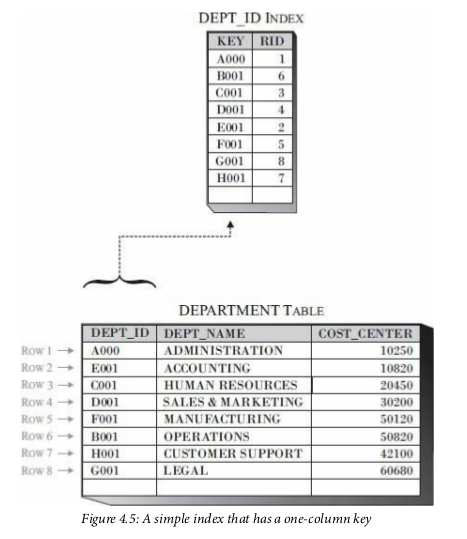
\includegraphics[scale=0.5]{index.png}
 
		\caption{Index that has a one-column key}
		\label{workloads}
		\end{figure}	
	\item Usage:
		\begin{itemize}
		\item fast, efficient method for locating specific rows of data in large tables
		\item logical ordering of the rows in a table
		\item enforce the uniqueness of records in a table
		\item force a table to use \textit{clustering} storage, which causes the rows of a table to be 
		physically arranged according to the ordering of their key column values.
		\end{itemize}
	\item tables that are used for data mining, business intelligence, business warehousing, and by
	applications that execute many (and often complex) queries but that rarely modify data are prime 
	candidates for index.
	\item tables in OLTP or environments where data throughput is high should use index sparingly or
	avoid them altogether.
	\end{itemize}
\item Aliases
	\begin{itemize}
	\item Similar to table or view, but cannot be used in the check condition of a check contraint
	or to reference a user-defined temporary table.
	\item Usage: allow to construct SQL statements in such a way that they are independent of the base
	tables or views they reference.
	\end{itemize}
\item Sequences
	\begin{itemize}
	\item PREVIOUS VALUE, NEXT VALUE
	\item Example scenario: An application running on a remote client needs to ensure that every new employee that joins the 
	company is assigned a unique, sequential employee number.
	\item "Change whether a sequence cycles", "establish new minimum and maximum sequence values", and "change the number of sequence numbers that are cached" can be done
	with ALTER SEQUENCE.
	\item "Change a sequence's data type" CANNOT done with ALTER SEQUENCE.
	\end{itemize}
\item Triggers
	\begin{itemize}
	\item an object that is used to define a set of actions that are to be executed whenever an insert,
	update, or delete operation is performed against a table or updatable view.
	\item Types:
		\begin{itemize}
		\item BEFORE triggers - The trigger's actions occur just before the triggering event takes place.
		\item AFTER triggers - The trigger's actions occur immediately after the triggering event takes
		place
		\item INSTEAD OF triggers - are executed in place of the trigger event (to ensure that 
		applications can perform insert, update, delete and query operations against an updatable
		view only)
		\end{itemize}
	\item Example scenario: An application running on a remote client needs to track every modification made to a 
	table that contains sensitive data.
	\end{itemize}
\item User-defined data types (UDTs)
	\begin{itemize}
	\item distinct data type - derived from one of the built-in data types that are provided with DB2
	\item {\color{green} structured data type} - contains multiple attributes, each of which has a name
	and data type of its own
	\end{itemize}
\item User-defined functions (UDFs)
	\begin{itemize}
		\item Example scenario: An application running on a remote client needs to be able to convert degress Celsius to degrees
		Fahrenheit and vice versa.
		\item category"
		\begin{itemize}
			\item SQL
			\item Sourced (Template): A function that is based on some other function that already exists.
			\item External Scalar: A function that is written using a high-level programming language.
			\item External Table: A function that returns a result data set in the form of a table.
			\item OLE DB External Table: A function that can access data from on Object Linking and 
				Embedding Database (OLE DB) provider and return a result data set in the form of a table.
		\end{itemize}
	\end{itemize}
\item Stored procedures
	\begin{itemize}
		\item Example scenario: An application running on a remote client needs to collect input values from a user, 
		perform a calculation using the values provided, and store the input data, along with the calculation
		results, in a base table.
		\item Category
		\begin{itemize}
			\item SQL: body is written entirely in SQL or SQL PL.
			\item {\color{red}External SQL}: body is written entirely in SQL, but that DB2 supports by generating 
				an associate C program for.
			\item External: body is written in a high-level programming language.
		\end{itemize}
	\end{itemize}
\item Packages
\end{itemize}

\subsubsection{System objects}
	\begin{itemize}
	\item Buffer pools
		\begin{itemize}
			\item One buffer pool is created automatically as part of the database creation process
			\item Once a page has been copied to a buffer pool, it remains there until the space it occupies is needed
		\end{itemize}
	\item Table spaces
		\begin{itemize}
		\item Every table space must have a buffer pool assigned to it
		\item DB2 for LUW:
			\begin{itemize}
			\item System Managed Space (SMS)
			\item Database Managed Space (DMS)
			\item Automatic Storage (AS)
			\end{itemize}
		\item DB2 for z/OS:
			\begin{itemize}
			\item Partitioned table space
			\item Segmented table space
			\item Universal table space
			\item Large object (LOB) table space
			\item XML table space
			\end{itemize}
		\end{itemize}
	\item The system catalog: DB2 updates the information stored in the system catalog whenever any
	of the following events occur:
		\begin{itemize}
		\item Database objects (ie. tables, index, views) are created, altered, or dropped
		\item Authorizations and privileges are granted or revoked
		\item Statistical information is collected
		\item Packages are bound to the database
		\end{itemize}
	\item Transaction log files
		\begin{itemize}
		\item write-ahead logging:
			\begin{itemize}
			\item insert operation - a record for the new row is written to the log buffer
			\item delete operation - a record containing the row's original values is written to the log
			buffer
			\item update operation - a record containing the row's original data, together with the 
			corresponding new data, is stored in the log buffer
			
			\begin{figure}[h]
			\centering
			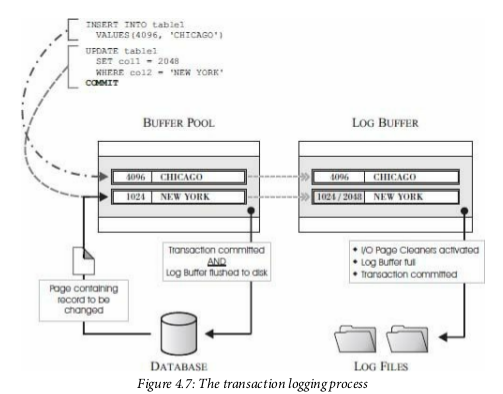
\includegraphics[scale=0.5]{transaction-logging.png}
 
			\caption{Transaction logging process}
			\end{figure}	
			\end{itemize}
		\end{itemize}
	\item The DB2 directory
	\item The bootstrap data set
	\item The data definition control supports (DDCS) database
	\item Resource limit facility tables
	\item The work file database
	\end{itemize}

\subsection{Creating a DB2 Database}
\begin{itemize}
\item DB2 for LUW:
	\begin{itemize}
	\item Syntax:
	\begin{verbatim}
	CREATE [DATABASE | DB] [DatabaseName]
		<AUTOMATIC STORAGE [YES | NO]>
		<ON [StoragePath, ...] <DBPATH [DBPath]>>
		<ALIAS [Alias]>
		<USING CODESET [CodeSet] TERRITORY [Territory]>
		<COLLATE USING [CollateType]>
		<PAGESIZE [4096 | Pagesize <k>]>
		<DFT_EXTENT_SZ [DefaultExtentSize]>
		<RESTRICTIVE>
		<CATALOG TABLESPACE [TS_Definition]>
		<USER TABLESPACE [TS_Definition]>
		<TEMPORARY TABLESPACE [TS_Definiton]>
		<WITH "[Description]">		
	\end{verbatim}
	\item Example:
		\begin{itemize}
		\item Requirement:
			\begin{itemize}
			\item Uses automatic storage
			\item Uses the paths "/mnt/fsystem1" and "/mnt/fsystem2" to store its data and metadata
			\item Recoginzes the United States and Canada code set
			\item Uses a collating sequence that is based on the United States and Canada code set
			\item Has a page size of 8 KB
			\end{itemize}
		\item SQL:
			\begin{verbatim}
			CREATE DATABASE sample
				ON /mnt/fsystem1, /mnt/fsystem2
				USING CODESET 1252 TERRITORY US
				COLLATE USING SYSTEM
				PAGESIZE 8192
			\end{verbatim}
		\end{itemize}
	\end{itemize}
\item DB2 for z/OS
\end{itemize}

\subsection{Establishing a Database Connection}
\begin{itemize}
\item connect example:
	\begin{verbatim}
	CONNECT TO sample USER db2user USING ibmdb2
	\end{verbatim}
\item Type 1 and Type 2 Connections
	\begin{figure}[H]
	\centering
	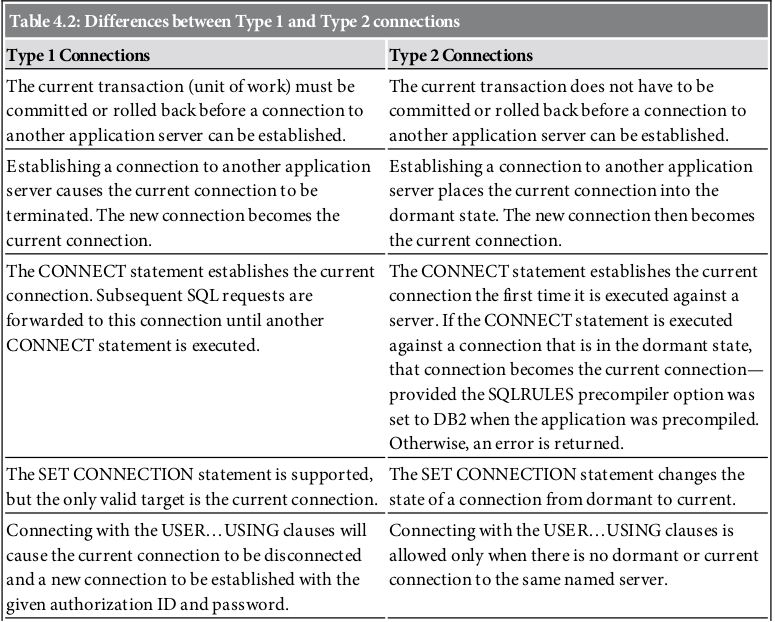
\includegraphics[scale=0.6]{type-connection.png}
	\caption{Difference between Type1 and Type2 connection}
	\end{figure}	
	\begin{itemize}
		\item Type 1 connections are used by default with DB2 LUW; Type 2 connections are used by default with DB2 z/OS.
		\item Type 2 connections allow a single transaction to connect to and work with multiple databases simultaneously.
		\item Type 1 connections allow a transaction to be connected to only one database at a time.
	\end{itemize}
\item DB2 Connect
	\begin{itemize}
	\item IBM DB2 Connect Application Server Edition
	\item IBM DB2 Connect Personal Edition
		\begin{itemize}
			\item makes DB2 data stored on System z, System i, and IBM Power Systems servers directly available to desktop applications
			\item enables applications to work transparently with data stored on multiple systems \textit{without using a gateway}
		\end{itemize}
	\item IBM DB2 Connect Enterprise Edition
		\begin{itemize}
			\item connects LAN-based systems and desktop applications to System z, System i, and IBM Power Systems databases
			\item host access can be consolidated through a gateway, making it easier to deploy web and multitier client/server applications
		\end{itemize}
	\item IBM DB2 Connect Unlimited Advanced Edition for System z
		\begin{itemize}
			\item makes it easy to access, manage, and optimize the performance of enterprise information, wherever it resides.
			\item Because it is licensed for unlimited deployment on authorized servers, this edition is cost-effective solution for organizations that
			use DB2 Connect extensively, especially where multiple applications are involved.
		\end{itemize}
	\item IBM DB2 Connect Unlimited Edition for System i
		\begin{itemize}
			\item integrates IBM System i data with client/server, web, mobile, and service-oriented architecture (SOA) applications.
			\item it delivers unified application development, integrated data, and pervasive data functionality to System i users.
		\end{itemize}
	\end{itemize}
\end{itemize}

\subsection{Temporal Data Management and Time Travel Tables}
\subsubsection{Basic Temporal Data Concepts}
\begin{itemize}
\item time period: {[date/time/timestamp, date/time/timestamp)}
\item system period: refers to the period in which a particular row is considered \textbf{current}. (
\textit{system time} is often associated with traching when changes are made to the state of a record)
\item application period: refers to the period in which a particular row is considered valid. (\textit{business time} (aka \textit{valid time}, \textit{application time}) is usually associated with
tracking the effective dates of certain business conditions.
\end{itemize}

\subsubsection{System-period temporal tables}
\begin{itemize}
\item table that maintains historical versions of its rows. 
\item must be associated with a history table
\item any time a row in a system-period temporal table is modified, DB2 automatically inserts a copy of
the original row into the corresponding history table.
\item Requirement:
	\begin{itemize}
		\item system/row time begin (\texttt{sys\_start}) (TIMESTAMP(12) data type)
		\item system/row time end (\texttt{sys\_end}) (TIMESTAMP(12) data type)
		\item transaction start-ID (\texttt{ts\_id}) (TIMESTAMP(12) data type): allow DB2 to capture the start times of transactions that perform update or delete operations on a particular row
		\item \texttt{PERIOD SYSTEM\_TIME} clause
	\end{itemize}
\item Example:
	\begin{itemize}
	\item Create a system-period temporal table named TAX\_INFO
    \begin{minted}[mathescape,
    	linenos,
    	numbersep=5pt,
    	gobble=2,
    	frame=lines,
    	framesep=2mm]{sql}
		CREATE TABLE tax_info
		 (taxpayer_id  CHAR(4) NOT NULL,
		  tax_amount   INT NOT NULL,
		  sys_start    TIMESTAMP(12) NOT NULL
						 GENERATED ALWAYS AS ROW BEGIN,
		  sys_end      TIMESTAMP(12) NOT NULL
						 GENERATED ALWAYS AS ROW END,
		  ts_id        TIMESTAMP(12) NOT NULL
						 GENERATED ALWAYS AS,
						 TRANSACTION START ID
						 IMPLICITLY HIDDEN
		  PERIOD SYSTEM_TIME (sys_start, sys_end))
    \end{minted}
    
    \item Create a history table named HIST\_TAX\_INFO with the same definition as the TAX\_INFO
    \begin{sqlcode}
    CREATE TABLE hist_tax_info LIKE tax_info
    \end{sqlcode}
    
    \item Establish a link between the system-period temporal table named TAX\_INFO and the history table
    named HIST\_TAX\_INFO
    \begin{sqlcode}
    	ALTER TABLE tax_info
    	 ADD VERSIONING
    	 USE HISTORY TABLE hist_tax_info
    \end{sqlcode}
%    \begin{lstlisting}[caption=hello]  % Start your code-block
%    
% CREATE TABLE tax_info
%  (taxpayer_id  CHAR(4) NOT NULL,
%   tax_amount   INT NOT NULL,
%   sys_start    TIMESTAMP(12) NOT NULL
%			      GENERATED ALWAYS AS ROW BEGIN,
%   sys_end      TIMESTAMP(12) NOT NULL
%				  GENERATED ALWAYS AS ROW END,
%   ts_id        TIMESTAMP(12) NOT NULL
%				  GENERATED ALWAYS AS,
%				  TRANSACTION START ID
%				  IMPLICITLY HIDDEN
%				  PERIOD SYSTEM_TIME (sys_start, sys_end))
%    \end{lstlisting}
\end{itemize}
\end{itemize}

\subsubsection{Application-period temporal tables}
\begin{itemize}
	\item a table that maintains "currently in effect" values of application data.
	\item Requirement:
		\begin{itemize}
			\item business time begin (\texttt{bus\_start})
			\item business time end (\texttt{bus\_end})
			\item \texttt{PERIOD BUSINESS\_TIME} clause
		\end{itemize}
	\item Example:
		\begin{itemize}
			\item Create an application-period temporal table named INVENTORY
			\begin{sqlcode}
			CREATE TABLE inventory
			 (item_id         CHAR(4) NOT NULL,
			  price           DOUBLE NOT NULL,
			  bus_start       DATE NOT NULL,
			  bus_end         DATE NOT NULL,
			 PERIOD BUSINESS_TIME (bus_start, bus_end),
			 PRIMARY KEY(item_id, BUSINESS_TIME WITHOUT OVERLAPS))
			\end{sqlcode}
		\end{itemize}
\end{itemize}

\subsubsection{Bitemporal tables}
\begin{itemize}
	\item combines the historical tracking of a system-period temporal table with the time-specific data storage capabilities of an application-period temporal table.
	\item a single table needs to maintain historical versions of its rows and keep track of data values that are currently considered valid.
	\item When querying a bitemporal table, you have the option of providing a system time-period 
	specification, a business time-period specification, or both, or neither.
	\item Example: 
		\begin{itemize}
			\item Create a bitemporal table named INVENTORY
\begin{sqlcode}
CREATE TABLE inventory
(item_id         CHAR(4) NOT NULL,
 price           DOUBLE NOT NULL,
 sys_start       TIMESTAMP(12) NOT NULL
				 GENERATED ALWAYS AS ROW BEGIN,
 sys_end         TIMESTAMP(12) NOT NULL
				 GENERATED ALWAYS AS ROW BEGIN,
 ts_id           TIMESTAMP(12) NOT NULL
 				GENERATED ALWAYS AS
 				TRANSACTION START ID, 
 bus_start       DATE NOT NULL,
 bus_end         DATE NOT NULL,
 PERIOD SYSTEM_TIME (sys_start, sys_end)
 PERIOD BUSINESS_TIME (bus_start, bus_end))
\end{sqlcode}
			\item Create a corresponding history table
\begin{sqlcode}
CREATE TABLE hist_inventory LIKE inventory
\end{sqlcode}
			\item Establish a link between \texttt{HIST\_INVENTORY} and \texttt{INVENTORY} table
\begin{sqlcode}
ALTER TABLE inventory
ADD VERSIONING
USE HISTORY TABLE hist_inventory
\end{sqlcode}
		\end{itemize}
\end{itemize}

\newpage
\section{Working with DB2 Data Using SQL}

\subsection{Objectives}
\begin{itemize}
\item Ability to use SQL to SELECT data from tables
\item Ability to use SQL to SORT or GROUP data
\item Ability to use SQL to UPDATE, DELETE, or INSERT data
\item Knowledge of transactions (ie. commit/rollback and transaction boundaries)
\item Ability to create and call an SQL supported procedure or a user defined function (understanding
of passing parameters and results)
\item Given an XQuery statement, knowledge to identify results
\item Knowledge of Temporal(Time Travel) Tables - System-period, Application-period, and Bi-temporal-
ability to query
\end{itemize}

\subsection{SELECT data from tables}
\subsubsection{FETCH FIRST - Getting a limited amount of data}
\begin{itemize}
\item To retrieve a specific number of rows from a table, use the SELECT statement with the FETCH FIRST
clause
\item Example: retrieve the first two rows from the \textit{sales} table:
\begin{sqlcode}
SELECT * FROM sales FETCH FIRST 2 ROWS ONLY
\end{sqlcode}
\end{itemize}

\subsubsection{Isolation clause - Accessing restricted data}
\begin{itemize}
\item To specify the isolation level a query is to be run under, and in some cases, to suggest the type
of lock DB2 should acquire and hold on the data being queried.
\item Example: retrieve uncommitted data from \textit{sales} table:
\begin{sqlcode}
SELECT * FROM sales WITH UR
\end{sqlcode}
\item Example: retrieve data from a table with minimal locking, use the FOR FETCH ONLY or FOR READ ONLY
\begin{sqlcode}
SELECT * FROM sales FOR FETCH ONLY
\end{sqlcode}
\end{itemize}
\subsubsection{WHERE clause - Restricting the result set}
\subsubsection*{WHERE clause}
\begin{itemize}
\item To restrict the data in the result set
\item Example: get all the employees from the \textit{employee} table who are hired after year 2005
and whose workdept is in 'AOO' and 'E21'
\begin{sqlcode}
SELECT * FROM employee WHERE YEAR(hiredate) > '2005' AND workdept IN ('AOO', 'E21')
\end{sqlcode}
\end{itemize}
\subsubsection*{Predicate}
\begin{itemize}
\item \textbf{LIKE} predicate: search for string patterns in column values
\item Example: find all employees whose first name starts with 'E' in the \textit{employee} table:
\begin{sqlcode}
SELECT * FROM employee WHERE firstnme LIKE 'E%'
\end{sqlcode}
\item \textbf{BETWEEN} predicate: specifying data ranges
\item Example: select employees whose hire date is between 1998 and 2000:
\begin{sqlcode}
SELECT firstnme FROM employee WHERE YEAR(hiredate) BETWEEN '1998' AND '2000'
\end{sqlcode}
\item \textbf{NULL} predicate: search for colmuns that have null values
\item Example: select all employees without a middle initial:
\begin{sqlcode}
SELECT firstnme FROM employee WHERE midinit IS NULL
\end{sqlcode}
\item \textbf{EXISTS} predicate: determine whether a particular value exists in a given result set
\item \textbf{IN} predicate
\end{itemize}

\subsubsection{DISTINCT clause - Eliminating duplicates}
\begin{itemize}
\item To eliminate duplicates from the final result set, use the SELECT DISTINCT clause
\item Example: select all the names of salespersons from the \textit{sales} table without duplicates:
\begin{sqlcode}
SELECT DISTINCT sales_person FROM sales
\end{sqlcode}
\end{itemize}

\subsubsection{GROUP BY clause - grouping data in result sets}
\subsubsection*{GROUP BY}
\begin{itemize}
\item Example: determine the average sales of a sales person in sales table:
\begin{sqlcode}
SELECT sales_person, AVG(sales) avg_sales FROM sales GROUP BY sales_person
\end{sqlcode}
\begin{verbatim}
SALES_PERSON   AVG_SALES
------------  -----------
GOUNOT                 3
LEE                    5 
LUCCHESSI              1
\end{verbatim}
\item Specify all columns that are not aggregated in GROUP BY clause
\end{itemize}
\subsubsection*{HAVING clause}
\begin{itemize}
\item \textbf{HAVING} clause: If you use the aggregate functins such as MIN() or MAX() to specify 
a condition, you must use the HAVING clause.
\item Example: determine the minimum and maximum salary paid for a job and the maximum salary is greater
than 27000
\begin{sqlcode}
SELECT job, MIN(salary), MAX(salary)
FROM employee
GROUP BY job
HAVING MAX(salary) >= 27000
\end{sqlcode}
\end{itemize}

\subsubsection*{GROUP BY ROLLUP clause}
\begin{itemize}
\item Example:
\begin{verbatim}
db2 => select job, sex, dec(avg(salary),9,2) from employee group by rollup (job, sex)

JOB      SEX 3
-------- --- -----------
-        -      58155.35
ANALYST  -      70213.33
CLERK    -      43876.25
DESIGNER -      57437.00
FIELDREP -      39274.00
MANAGER  -      88142.14
OPERATOR -      37898.33
PRES     -     152750.00
SALESREP -      56500.00
ANALYST  F      70213.33
CLERK    F      42315.00
CLERK    M      44396.66
DESIGNER F      58317.50
DESIGNER M      56850.00
FIELDREP F      35370.00
FIELDREP M      40250.00
MANAGER  F      94723.33
MANAGER  M      83206.25
OPERATOR F      38575.00
OPERATOR M      36545.00
PRES     F     152750.00
SALESREP F      46500.00
SALESREP M      66500.00

23 record(s) selected.
\end{verbatim}
\end{itemize}

\subsubsection*{GROUP BY CUBE clause}
\begin{itemize}
	\item Example:
	\begin{verbatim}
	db2 => select job, sex, dec(avg(salary),9,2) from employee group by rollup (job, sex)
	
	JOB      SEX 3
	-------- --- -----------
	-        F      63243.68
	-        M      53951.95
	-        -      58155.35
	ANALYST  -      70213.33
	CLERK    -      43876.25
	DESIGNER -      57437.00
	FIELDREP -      39274.00
	MANAGER  -      88142.14
	OPERATOR -      37898.33
	PRES     -     152750.00
	SALESREP -      56500.00
	ANALYST  F      70213.33
	CLERK    F      42315.00
	CLERK    M      44396.66
	DESIGNER F      58317.50
	DESIGNER M      56850.00
	FIELDREP F      35370.00
	FIELDREP M      40250.00
	MANAGER  F      94723.33
	MANAGER  M      83206.25
	OPERATOR F      38575.00
	OPERATOR M      36545.00
	PRES     F     152750.00
	SALESREP F      46500.00
	SALESREP M      66500.00
	
	25 record(s) selected.
	\end{verbatim}
\end{itemize}


% Generate the bibliography.
%\bibliography{latex-sample}
%\bibliographystyle{unsrt}


\end{document}
